\documentclass[10pt,a4paper]{article}
% WSPR Logger mobile app user guide. Built with:  pdflatex mobile_guide.tex  (three times for the contents)
% The screenshots are in guide_img_m/ (taken from the running phone view /app with the station's own databases).
\usepackage[T1]{fontenc}
\usepackage[utf8]{inputenc}
\usepackage{mathptmx}
\usepackage[scaled=.92]{helvet}
\usepackage{courier}
\usepackage{microtype}
\usepackage[a4paper,margin=2.0cm,top=2.3cm,bottom=2.2cm,headsep=0.5cm]{geometry}
\usepackage{graphicx}
\usepackage{xcolor}
\usepackage{booktabs}
\usepackage{tabularx}
\usepackage{array}
\usepackage{enumitem}
\usepackage{caption}
\usepackage{float}
\usepackage{fancyhdr}
\usepackage{textcomp}
\usepackage{amsmath}
\usepackage{amssymb}
\usepackage{tikz}
\usetikzlibrary{arrows.meta,positioning}
\usepackage[hidelinks]{hyperref}

\definecolor{accent}{HTML}{0369A1}
\definecolor{boxbg}{HTML}{F1F6FA}
\definecolor{warnbg}{HTML}{FFF7E8}
\definecolor{warn}{HTML}{B45309}
\captionsetup{font=small,labelfont=bf,labelsep=period,justification=justified,singlelinecheck=false}
\setlist{itemsep=1.5pt,topsep=3pt,parsep=0pt}
\setlength{\parindent}{0pt}
\setlength{\parskip}{4.5pt plus 1pt}
\renewcommand{\arraystretch}{1.15}
\setcounter{tocdepth}{2}
\pagestyle{fancy}
\fancyhf{}
\fancyhead[L]{\small\itshape WSPR Logger --- the phone view (mobile app)}
\fancyhead[R]{\small\itshape Mobile app user guide, version 1.8 --- November 2026}
\fancyfoot[C]{\small\thepage}
\renewcommand{\headrulewidth}{0.3pt}
\hypersetup{pdftitle={WSPR Logger - Mobile app user guide},pdfauthor={Otso Laakso, OH2GAX}}

\newcommand{\km}{\,km}
\newcommand{\dB}{\,dB}
\newcommand{\MHz}{\,MHz}
\newcommand{\ui}[1]{\textsf{\small #1}}            % a word on the screen: button, switch, card title
\newcommand{\lead}[1]{\textbf{#1}\enspace}           % run-in paragraph head
\newcommand{\fig}[3]{\begin{figure}[H]\centering\includegraphics[width=#2\textwidth]{guide_img_m/#1}\caption{#3}\end{figure}}
\newcommand{\figpair}[5]{\begin{figure}[H]\centering
  \begin{minipage}[t]{0.485\textwidth}\centering\includegraphics[width=\textwidth]{guide_img_m/#1}\end{minipage}\hfill
  \begin{minipage}[t]{0.485\textwidth}\centering\includegraphics[width=\textwidth]{guide_img_m/#2}\end{minipage}
  \caption{#5}\label{#3}\end{figure}}
\newcommand{\infobox}[2]{\par\smallskip\noindent\fcolorbox{accent!60}{boxbg}{\begin{minipage}{\dimexpr\textwidth-2\fboxsep-2\fboxrule\relax}\small
  \textbf{#1}\enspace #2\end{minipage}}\par\smallskip}
\newcommand{\warnbox}[2]{\par\smallskip\noindent\fcolorbox{warn!60}{warnbg}{\begin{minipage}{\dimexpr\textwidth-2\fboxsep-2\fboxrule\relax}\small
  \textbf{#1}\enspace #2\end{minipage}}\par\smallskip}
% "How to read" block of an Analysis card
\newenvironment{reading}{\par\begin{description}[leftmargin=0pt,labelsep=0.4em,itemsep=2pt,font=\normalfont\bfseries]}{\end{description}\par}

% phone screenshots side by side: \phones{w}{a}{b}{c}{caption} (c may be empty)
\newcommand{\phone}[2]{\fbox{\includegraphics[width=#1\textwidth]{guide_img_m/#2}}}
\newcommand{\phones}[5]{\begin{figure}[H]\centering\setlength{\fboxsep}{0pt}\setlength{\fboxrule}{0.3pt}%
  \phone{#1}{#2}\hfill\phone{#1}{#3}\ifx&#4&\else\hfill\phone{#1}{#4}\fi\caption{#5}\end{figure}}
\newcommand{\phonetwo}[4]{\begin{figure}[H]\centering\setlength{\fboxsep}{0pt}\setlength{\fboxrule}{0.3pt}%
  \phone{#1}{#2}\hspace{1.2cm}\phone{#1}{#3}\caption{#4}\end{figure}}
\begin{document}
\thispagestyle{plain}
\begin{center}
{\small WSPR Logger project \quad$\cdot$\quad Mobile app user guide, version 1.8 \quad$\cdot$\quad 9 November 2026}\par\vspace{10pt}
{\LARGE\bfseries WSPR Logger on your phone}\par\vspace{5pt}
{\large\bfseries The mobile app: the live map, propagation, replay,\\ history, analysis and the car's track in one hand}\par\vspace{8pt}
{\normalsize Otso Laakso (OH2GAX)}\par
{\small \url{https://wspr.oh2gax.org/app} \quad$\cdot$\quad \url{https://github.com/oh2gax/wspr_logger}}
\end{center}
\vspace{2pt}

\infobox{In short.}{The phone view (the ``mobile app'') shows the same data as the full WSPR Logger page, made for a phone screen: \textbf{one view at a time, filling the screen}, and \textbf{every choice in the menu} behind the \ui{$\equiv$} button at the top left. There is nothing to install: open \url{https://wspr.oh2gax.org/app} in the phone's browser, and if you like, add it to the home screen so that it opens like an app (Section~\ref{sec:open}). It has nine views:
\begin{itemize}[leftmargin=1.2em]
\item \textbf{Live map} and \textbf{Now} --- where the car is, how well it is heard, the space weather (Sections~\ref{sec:map}--\ref{sec:now});
\item \textbf{Reporters} and \textbf{MUF graph} --- the stations of the last hour and the ionosonde (Sections~\ref{sec:rep}--\ref{sec:muf});
\item \textbf{Replay}, \textbf{History} and \textbf{Statistics} --- any earlier moment or day (Sections~\ref{sec:replay}--\ref{sec:stats});
\item \textbf{Analysis} --- the full page's Propagation Analysis, card under card (Section~\ref{sec:analysis});
\item \textbf{WPRS} --- the car's drives and trips as tracks (Section~\ref{sec:wprs}).
\end{itemize}
The user interface is the same as in the author's MODE-S Wind phone view, so if you know one, you know the other. What the numbers and charts \emph{mean} is explained in the \emph{WSPR Logger --- User guide}; this guide tells where to find them on the phone.}

\infobox{About the figures.}{The screenshots were taken on a phone-sized screen (390\,$\times$\,844 points) with the station's own data as it was on 6 November 2026 at 14:20~UTC. On the maps of the figures the background is a plain outline of the continents; in the app it is a detailed street map. The numbers on your screen will differ, because the data grows every ten minutes. \textbf{Version history:} 1.0, 7 November 2026, first version; 1.1, the same day: the Analysis periods 7\,d and 14\,d and the opening at 14 days, the all-time Best DX without implausible reports, country names from the locator, the phone's Back returning to the previous view, and the replayed moment in the top-bar clock; 1.2, 8 November 2026: the solar card and the MUF card on the Live map; 1.3, 9 November 2026: the MUF card's range; 1.4, the same day: the Typical day in the Now view and as a Live map card; 1.5: foF2 on the MUF card, the age label at the car shortened to \emph{N min ago}; 1.6: \ui{Remember position} for the Live map; 1.7: propagation compared with usual and the transmitter warning; 1.8: unusual DX openings.}

{\small\tableofcontents}

\newpage
\section{Opening the app}\label{sec:open}

\lead{The address.} Open \url{https://wspr.oh2gax.org/app} in the phone's browser (Safari, Chrome, Firefox, Samsung Internet \dots). On the full page the same link is in the top-left corner, under \ui{What's new}: \ui{Phone app}. The full page itself still works on a phone, but its menu and floating panels are made for a mouse and a wide screen; the phone view is easier to use with one thumb.

\lead{On the home screen.} The app can be added to the home screen like any web app. It then opens full screen, without the browser's address bar, with its own icon (a green beacon sending blue waves):
\begin{itemize}[leftmargin=1.2em]
\item \textbf{iPhone, iPad} (Safari): the Share button $\rightarrow$ \ui{Add to Home Screen} $\rightarrow$ \ui{Add}.
\item \textbf{Android} (Chrome): the $\vdots$ menu $\rightarrow$ \ui{Add to Home screen} or \ui{Install app}.
\end{itemize}
Nothing is installed from an app store and no account is needed; the app is the web page.

\lead{What is kept on the phone.} The view you were on, the switches and choices of the menu, the map zoom, the theme and the version of the notes you have read are stored in the browser (its local storage). The next time you open the app it continues where you left it. In a private (incognito) window the browser forgets them when the window closes.

\lead{Always up to date.} When a new version of the WSPR Logger is put on the server, an open app notices it the next time you come back to it, and reloads itself (Section~\ref{sec:fresh}). You never need to clear the browser's cache.

\section{The screen}\label{sec:screen}
\phones{0.31}{d_map.jpg}{d_menu.jpg}{d_menu_gen.jpg}{The Live map view (left), the menu opened with \ui{$\equiv$} (middle), and the General section at the bottom of the menu (right).}

\lead{The top bar.} From left to right:
\begin{itemize}[leftmargin=1.2em]
\item \ui{$\equiv$} opens the menu. A \textbf{red dot} on it means there are new notes in \ui{What's new} that you have not read yet;
\item the \textbf{title} of the view, and under it a short subtitle: the callsign, the latest locator and the band on the live views, the shown day on Replay and History;
\item the \textbf{UTC clock}. All times in WSPR Logger are UTC (Finnish time is UTC\,+\,2, in summer UTC\,+\,3);
\item the \textbf{theme button}. Its icon shows the setting in use: a moon for Dark, a sun for Light, a half-filled circle for Auto (follows the phone's own light/dark setting, also while the app is open). A tap steps Dark $\rightarrow$ Light $\rightarrow$ Auto $\rightarrow$ Dark; a short note under the button names the new setting. The setting is shared with the full page in the same browser;
\item the \textbf{status dot} of the beacon: \textbf{green} when the newest transmission was heard less than 20 minutes ago, \textbf{amber} up to 2 hours, \textbf{red} beyond (the car is parked with the transmitter off, or nobody hears it). The same text is in the menu under \ui{General}.
\end{itemize}

\lead{The views.} Each view fills the screen below the top bar. Long views (Now, Reporters, History, Analysis, WPRS) scroll up and down; the map views fill the screen exactly. Turn the phone sideways for a wider map: on Replay the time panel then moves beside the map (Figure~\ref{fig:land}).

\lead{The phone's Back.} Back works as in an app: it closes the menu or a sheet (What's new, User guides, About) when one is open, and otherwise returns to the view you were in before --- e.g.\ from Replay opened in History back to that day's History. In the first view you opened, Back leaves the app.

\section{The menu}\label{sec:menu}
The menu slides in from the left. Tap \ui{$\times$}, the darkened page on the right, or the phone's Back gesture to close it.

\lead{The view tiles.} The nine views are tiles at the top. A tap opens the view and closes the menu; the tile of the shown view is highlighted.

\lead{The options.} Under the tiles each view has a folding section with its options, e.g.\ \ui{Live map options}. The section of the shown view opens by itself and its title is blue; the others stay folded but can be opened (and changed) at any time. Below the choices each section has a short explanation of the view. The options are
\begin{itemize}[leftmargin=1.2em]
\item \textbf{chips} --- a row of buttons of which one is on (filled blue), e.g.\ the range of the MUF graph;
\item \textbf{switches} --- on (blue, knob right) or off, e.g.\ \ui{Reporter arcs} on the map;
\item \textbf{date steppers} --- \ui{$\langle$}\,date\,\ui{$\rangle$}: the arrows step a day, a tap on the date opens the phone's calendar.
\end{itemize}
Every choice takes effect at once and is remembered on the phone.

\lead{General.} The last section has \ui{What's new} (the short notes of each version, newest first, the same as on the full page), \ui{About} (the station and the software) and \ui{User guides} (the PDF guides of the Guides list, this one among them), and the \ui{Full site} link. What's new is also at the top of the menu next to the title. These open as a full-screen sheet; its top row has buttons for the other two, and \ui{$\times$} or Back closes it.

\phones{0.31}{d_menu_map.jpg}{d_menu_replay.jpg}{d_news.jpg}{Options of the Live map (left) and of Replay (middle) in the menu, and What's new (right).}

\section{The views}

\subsection{Live map}\label{sec:map}
The car's latest position on the map, as on the full page's Live Map.
\begin{itemize}[leftmargin=1.2em]
\item The \textbf{dot} is the latest fix: green, or red when nothing has been heard for an hour. Its \textbf{label} tells how old the fix is --- green up to 25 minutes (a transmission every 10 minutes plus the upload delay), amber to an hour, red beyond. Tap the dot for the locator, time, stations and farthest station.
\item The \textbf{status card} at the bottom: the locator, the age of the fix, the band, the \textbf{propagation estimate} with its bar and, below it, how that compares with usual for the hour (Section~\ref{sec:now}), the number of stations that heard the latest transmission, the farthest one and the time.
\item The \textbf{solar card} (option, off at first): the space weather of the Now view (Section~\ref{sec:now}) over the map --- SFI, K and A index, X-ray, Bz, solar wind, aurora, proton flux, foF2 and the Juliusruh MUF, in the same colours, with the time of the last update.
\item The \textbf{MUF card} (option, off at first): the MUF graph of Section~\ref{sec:muf} in small --- the MUF for a 3\,000\,km hop (the blue line, left scale) and the stations that heard each transmission (the green bars, right scale) over the last 24 hours, with the latest MUF and its time in the corner. \ui{MUF card range} in the options sets the period: \ui{24 h} (every reading and transmission), \ui{2 days}, \ui{3 days} or \ui{1 week} (by the hour: the hour's mean MUF and its most reporters, with the weekday at each midnight); hours without data stay empty. The option \ui{foF2 on MUF card} adds the Juliusruh \textbf{foF2} as an amber line on the same MHz scale (the MUF over 3\,000\,km is about three times foF2; foF2 is stored from November 2026). It is fetched again every 5 minutes for 24 hours, every 15 minutes for two or three days and every 30 minutes for a week.
\item The \textbf{Typical day card} (option, off at first): the Typical day of the Now view (Section~\ref{sec:now}) in small --- how many stations usually hear the car at each UTC hour (the blue line, with the middle half of the days shaded) and today (the orange line). The corner compares the latest hour with the usual, for example \emph{14 UTC: 116, usually 102}. Its period, \ui{Typical day over} (7, 14, 30 or 90 days), is the same setting as in the Now options.
\item \textbf{$+$ / $-$} zoom (or pinch), the \textbf{house button} brings the map back to the car.
\end{itemize}
The cards stand at the bottom of the map --- solar, MUF, typical day and status from the top; with the phone turned sideways they stand side by side (Figure~\ref{fig:cards}). They let taps through, so the map under them can still be moved.

\textbf{Options:} \ui{Position trail} (the day's positions as a dashed line), \ui{Last fix label}, \ui{Reporter arcs} (a great-circle line to every station that heard the beacon in the last 60 minutes --- the stronger the signal, the brighter and thicker the line; tap a station's dot for its callsign, grid, SNR, distance and country), \ui{Day / Night} (the night side shaded and the grey line dashed, moved every minute), \ui{Status card}, \ui{Solar card}, \ui{MUF card} with its \ui{MUF card range} and \ui{foF2 on MUF card}, \ui{Typical day card} with \ui{Typical day over}, \ui{Follow beacon} (the map moves with each new fix) and \ui{Remember position} (the map opens where you left it instead of at the car; the zoom is always remembered, and the house button still brings you back to the car). The view is refreshed every minute.

\begin{figure}[H]\centering\setlength{\fboxsep}{0pt}\setlength{\fboxrule}{0.3pt}
\begin{minipage}[b]{0.233\textwidth}\centering\fbox{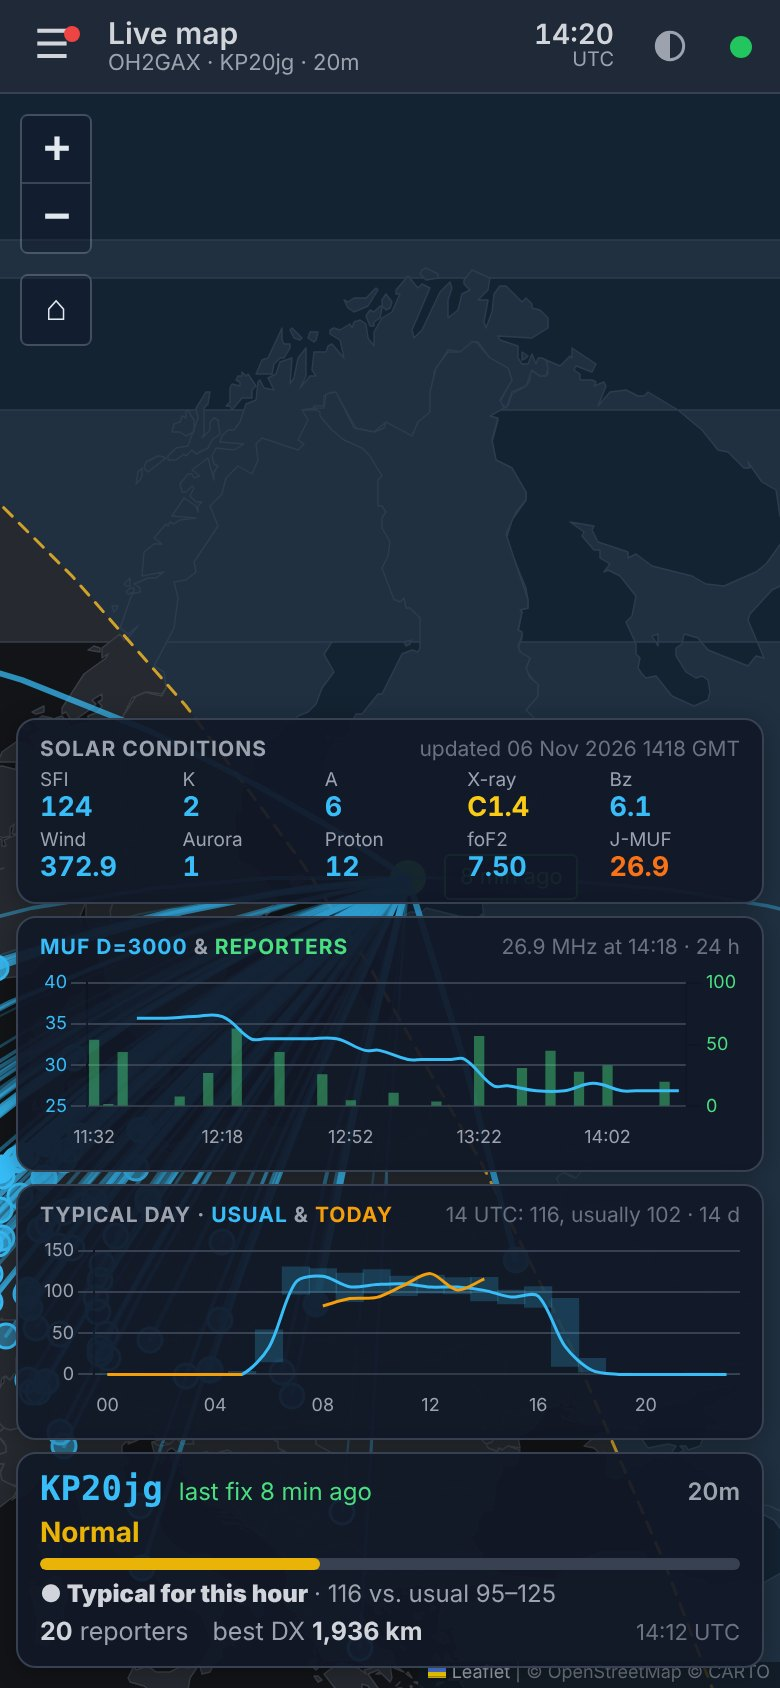
\includegraphics[width=0.99\linewidth]{guide_img_m/d_map_cards.jpg}}\end{minipage}\hfill
\begin{minipage}[b]{0.715\textwidth}\centering\fbox{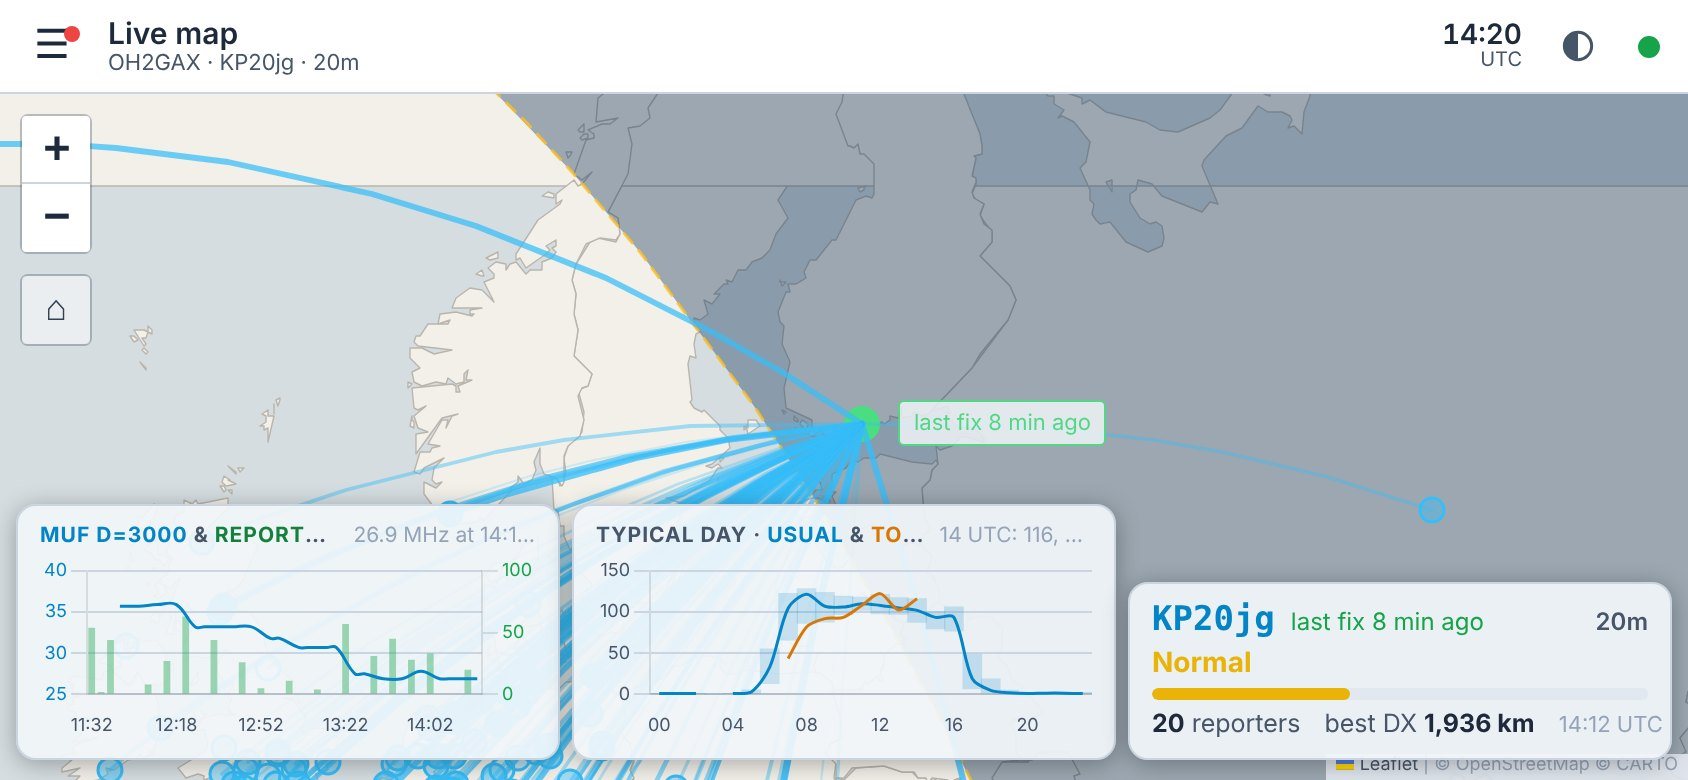
\includegraphics[width=0.99\linewidth]{guide_img_m/d_map_cards_land.jpg}}\end{minipage}
\caption{The Live map with all four cards upright in the dark theme (left), and sideways in the light theme with the MUF and Typical day cards (right).}\label{fig:cards}\end{figure}

\subsection{Now}\label{sec:now}
\phones{0.31}{d_now.jpg}{d_rep.jpg}{d_rep2.jpg}{Now (left); Reporters: the list (middle) and, further down, the countries and the SNR distribution (right).}
The present situation in numbers, card under card:
\begin{description}[leftmargin=0pt,labelsep=0.4em,itemsep=2pt,font=\normalfont\bfseries]
\item[Propagation] the number of stations that heard the latest transmission, as a word and a bar: Very low ($\le 5$), Low ($\le 10$), Normal ($\le 20$), Good ($\le 40$), Very good ($\le 60$), Extremely good ($\le 100$), Exceptional. \textbf{\& DX} is added when two or more of the stations heard in the last hour are beyond 6\,000\,km, and \textbf{HIGH MUF} when the Juliusruh MUF is above 28\,MHz. \emph{No propagation} means nothing was heard for an hour (at an hour when the band is usually open, judged from the last 30 days, the app says \emph{No propagation or TX Fail}, because silence then is suspicious).
\item[Compared with usual] under the bar: the stations heard in the last 60 minutes against the 30 days before today at the same UTC hour and a similar MUF --- \emph{Much below usual}, \emph{Below usual}, \emph{Typical for this hour}, \emph{Above usual} or \emph{Exceptional for this hour} --- with a gauge of the usual range (dark: the middle half, light: 10--90\,\%, line: the median, dot: now). The level above says \emph{how many}, this line \emph{how good for the hour}. \emph{No reports for 20 min} (amber) means nobody heard the last two polls at an hour when the band is usually open: \emph{transmitter off? Check the battery}. \emph{Transmitter back on}: the comparison returns an hour after a break. The status card on the Live map shows the same in one line.
\item[Unusual openings] a purple \emph{$\bigstar$ Unusual opening} line when a region beyond 6\,000\,km is heard at an hour when it is seldom heard at this time of year (on fewer than 2.5\,\% of days), or a green \emph{$\blacktriangle$ Unusually strong} line when a usual region is heard by many more stations than ever usual; with the stations' callsigns. On the Live map those stations' arcs turn the same colour, and the status card shows the line too. The Analysis view lists every such event of the history in the card \emph{Unusual DX openings}, with $\blacktriangleright$ to replay it.
\item[Position] the locator, the coordinates, the stations and farthest station of the latest transmission, its time and the age of the fix.
\item[Today / Last hour] the transmissions heard, the best distance and the most stations of one transmission --- for today (UTC) or the last 60 minutes (option \ui{Spots of}).
\item[Solar conditions] the space weather of hamqsl.com and the Juliusruh ionosonde, coloured as on the full page's Solar panel: green and blue quiet or good, yellow, orange and red increasingly disturbed, purple extreme. For the MUF the colours go the other way --- the higher, the more the band is open.
\item[Typical day (UTC)] the Analysis page's \emph{Typical day} chart: for each UTC hour the median number of stations heard in 60 minutes (blue line) and the range of the middle half of the days (shaded), over the last 7, 14 (at first), 30 or 90 days (option \ui{Typical day over}), with today in orange. If the orange line runs above the shaded range the band is better than usual at that hour. Tap the chart for an hour's values (Figure~\ref{fig:nowtyp}).
\item[Compared with history] the Analysis page's \emph{Right now} card over the last 90 days: how many stations heard the beacon in the last hour, how many are typical at this hour of the day and at a similar MUF, and the verdict \emph{Better than usual}, \emph{Typical} or \emph{Below usual}.
\end{description}
\phones{0.31}{d_now_typ.jpg}{d_menu_now.jpg}{l_now_typ.jpg}{The Typical day card in the Now view (left), the Now options with \ui{Typical day over} (middle), and the same in the light theme (right).\label{fig:nowtyp}}

\subsection{Reporters}\label{sec:rep}
The stations that heard the beacon in the last 60 minutes (the full page's Reporter list, Reporter countries and histogram), with a \textbf{search} field at the top that matches the callsign, the grid or the country anywhere (``germ'' finds every German station). Each row shows the callsign, the grid, the country, the SNR and the distance; distances beyond 6\,000\,km are bold.
\textbf{Options:} \ui{Sort by} SNR, distance, callsign or country; \ui{Distribution of} SNR or distance; and which \ui{Sections} are shown: the list, the countries (one bar per country, the most stations on top) and the distribution chart. The countries and the chart follow the search, so a search for a country shows its own SNR distribution.

\subsection{MUF graph}\label{sec:muf}
\phones{0.31}{d_muf.jpg}{d_replay.jpg}{d_hist.jpg}{MUF graph (left), Replay (middle) and History (right).}
The full page's MUF panel, as large as the screen: the \textbf{line} is the maximum usable frequency for a 3\,000\,km hop measured by the Juliusruh ionosonde (MHz, left scale), the \textbf{bars} the stations that heard each transmission (right scale). When the MUF climbs well above 14\,MHz the 20\,m band opens and the bars grow; in the evening both fall together. Tap the chart for the values of a moment. \textbf{Options:} \ui{Range} 24\,h, 2 days, 3 days or 1 week.

\subsection{Replay}\label{sec:replay}
The full page's History Player: the snapshots stored by the logger, about one every ten minutes, each with the stations that had heard the beacon in the preceding hour.
\begin{itemize}[leftmargin=1.2em]
\item The \textbf{map} shows the car where it was at that moment, the arcs to the stations of the snapshot and the night side of that moment, and the day's path as a grey dashed line.
\item The \textbf{panel} below it: the time, the propagation estimate of that moment and the number of stations heard, the snapshot number (e.g.\ 96\,/\,96), the \textbf{slider} (drag it through the day), and the buttons \ui{$\langle$ day} and \ui{day $\rangle$} (the previous / next day with data), \ui{$-$10m} and \ui{$+$10m} (one snapshot back / forward) and \ui{$\blacktriangleright$} (play; \ui{\textbf{II}} pauses).
\end{itemize}
While Replay is shown, the clock in the top bar gives the replayed moment instead of the present time, in amber and labelled \ui{REPLAY}. Replay opens at the newest snapshot. \textbf{Options:} the \ui{Date (UTC)} with its stepper (a date without data shows the nearest earlier day with data), the playing \ui{Speed} (1--16 snapshots a second), and the switches \ui{Reporter arcs} and \ui{Day / Night}.

\lead{Opened from other views.} A tap on a row of \textbf{History}, on \ui{$\blacktriangleright$} in an \textbf{Analysis} table (storm days, farthest reporters, unusual days) or on \ui{Replay} in \textbf{WPRS} opens Replay at that very moment; the phone's Back returns to where you came from.

\begin{figure}[H]\centering\setlength{\fboxsep}{0pt}\setlength{\fboxrule}{0.3pt}
\fbox{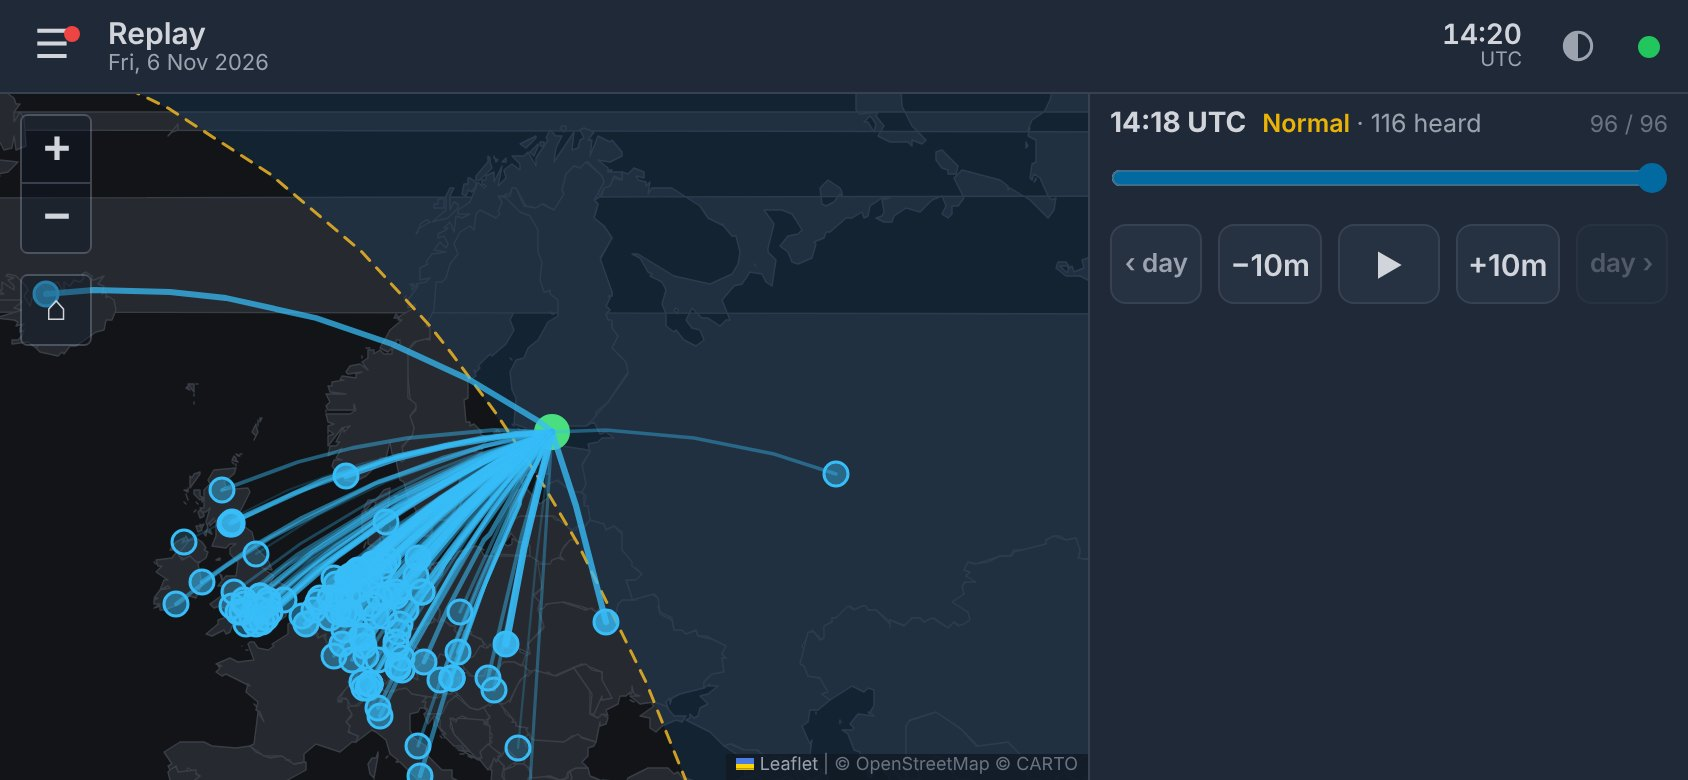
\includegraphics[width=0.66\textwidth]{guide_img_m/d_replay_land.jpg}}
\caption{Replay with the phone turned sideways: the panel beside the map.}\label{fig:land}\end{figure}

\subsection{History}\label{sec:history}
One UTC day, as the full page's History and Statistics pages together. At the top: \ui{$\langle$}\,date\,\ui{$\rangle$} and \ui{Today}. Then
\begin{itemize}[leftmargin=1.2em]
\item the day's numbers: transmissions heard (\emph{spots}), the most stations of one transmission, the best distance, the average number of stations, and the first and last transmission heard;
\item a \textbf{map} of the day's positions (green the first, blue the last; tap one for its details; the house button fits the whole day);
\item a \textbf{chart}: the bars are the stations of each transmission, the line the farthest station;
\item every transmission of the day, newest first: time, locator, stations, farthest distance. \textbf{Tap a row to open that moment in Replay.}
\end{itemize}
\textbf{Options:} the \ui{Map} and the \ui{Chart} can be switched off for a shorter page.

\subsection{Statistics}\label{sec:stats}
\phones{0.31}{d_stats.jpg}{d_an0.jpg}{d_an1.jpg}{Statistics (left); Analysis: the top of the view, here 14 days (middle) and further down the band-open heatmap and the DX outlook (right).}
The \textbf{all-time records}: the transmissions heard so far, the active days, the best distance and the most stations (with the day each record was set), and the first and last transmission ever heard. Below them a \textbf{chart day by day}: the bars are each day's best distance, the line the most stations of one transmission that day. \textbf{Tap a day in the chart to open it in History.} \textbf{Options:} \ui{Range} 30 days, 90 days or all.

\subsection{Analysis}\label{sec:analysis}
The full page's Propagation Analysis page, with all its cards one under the other in the same order: the summary, Right now, the ionosonde view, the band-open heatmap, the DX outlook, the typical day, the space-weather charts, the grey-line windows, the compass chart of where you are heard, the distance distribution, band opening and closing, season against season, stations per month, signal strength by hour and by distance, unusual days, the storm days, the farthest and the most loyal stations. \emph{How to read each card is explained in Section~5 of the WSPR Logger User guide} (open it from \ui{General} $\rightarrow$ \ui{User guides}).

The \textbf{period} buttons (7\,d, 14\,d, 30\,d, 90\,d, 6\,m, 1\,yr, All) are at the top of the view and also in the menu (\ui{Analysis options} $\rightarrow$ \ui{Period}); the two stay in step. The buttons inside the cards (e.g.\ \ui{Reporters} / \ui{Farthest km} of the heatmap, the periods of the ionosonde view) work as on the full page. Tap a chart or a heatmap cell for its values. Wide tables (the DX outlook) scroll sideways within their card.

\infobox{Opening and changing the period.}{The view opens at the last 14 days, which the server prepares in advance every ten minutes, so the cards appear at once. When those days hold no reports (the transmitter is off, usually from November to March), it opens at the first longer period that has some and says so beside the dates. Another period is computed when you choose it and then kept for ten minutes: the first time it can take a few seconds --- the old cards stay, dimmed, with \emph{Loading \dots} beside the buttons. The rest of the app is not slowed down meanwhile.}

\phones{0.31}{d_an2.jpg}{d_wprs.jpg}{l_an.jpg}{Analysis: where you are heard (left); WPRS with a drive on the map (middle); Analysis in the Light theme (right).}

\subsection{WPRS}\label{sec:wprs}
The full page's WPRS page (Whisper Position Reporting System): the positions in the transmissions turned into tracks of the car.
\begin{itemize}[leftmargin=1.2em]
\item The \textbf{map} at the top shows the chosen day or trip: the Maidenhead squares the car was in (darker: more fixes), the path as a dashed line, the start (green), the end (red) and the home square (red ring). The orange line and ring follow the fix shown below.
\item The \textbf{panel}: the time, locator and stations of the shown fix, the \textbf{slider} over the fixes, \ui{$\blacktriangleleft\blacktriangleleft$} (to the start), \ui{$\langle$} / \ui{$\rangle$} (one fix), \ui{$\blacktriangleright$} (play) and \ui{Replay} (opens the shown fix's moment in Replay). Under the buttons a summary: fixes, squares, how far the car moved, the path length and the greatest distance from home.
\item The \textbf{list} below: the logged \emph{days} with movement (each with a bar of how far it went), or the \emph{trips} beyond 25\,km from home. Tap one to show it on the map; the view scrolls back to the top.
\end{itemize}
\textbf{Options:} \ui{List} Days or Trips; \ui{Days with movement or distance from home of at least} any change of square, 5, 10, 25, 100, 150 or 200\,km (the same setting as on the full page); \ui{Track of} 1--7 days from the chosen day (a trip sets it to its own length); and the playing \ui{Speed}.

\section{Staying up to date}\label{sec:fresh}
\lead{Refreshing.} The Live map, Now and Reporters fetch new data every minute, the MUF graph every ten minutes and the Live map's MUF card every 5 to 30 minutes, depending on its range. Only the view on the screen is refreshed, and \textbf{nothing at all while the app is not on the screen} (the phone is locked or another app is open), so the app uses no data in the background. The other views load when you open them or change a date or an option.

\lead{Coming back.} When you return to the app it refreshes the shown view at once. If it has been away for more than an hour, or a new version has been put on the server meanwhile, it reloads itself completely --- the view and all your choices stay. A new version also brings a red dot to \ui{$\equiv$} and \ui{What's new} until you have read the notes (the full page then no longer marks them either, in the same browser).

\lead{Data use.} A refresh of the Live map is about 1\,kB, or about 12\,kB with the reporter arcs on; the solar card adds under 1\,kB a minute, the Typical day card or chart about 2\,kB every five minutes and the MUF card about 12\,kB per day of its range (every 5 minutes for 24 hours, every 30 for a week); the map tiles are loaded as you move the map and kept by the browser. The Analysis view loads about 60--100\,kB once per period, Replay about 200\,kB per day. The program itself (with the map and chart libraries, about 0.5\,MB) is loaded once and then kept by the browser.

\section{The phone view and the full page}
\begin{table}[H]\small\centering
\begin{tabularx}{\textwidth}{@{}>{\raggedright}p{3.1cm}>{\raggedright\arraybackslash}X@{}}
\toprule
\textbf{Full page} & \textbf{Phone view} \\ \midrule
Live Map: map and layers & \textbf{Live map}: trail, fix label, reporter arcs (Reporter Plot) and Day/Night as switches; the overlay as the status card; the Solar Conditions panel and the MUF panel also as cards over the map \\
Left pane: Locator, Propagation, Today / 1h & \textbf{Now} \\
Solar Conditions panel & \textbf{Now} $\rightarrow$ Solar conditions \\
Reporter list, countries, histogram & \textbf{Reporters} (with a search) \\
MUF panel & \textbf{MUF graph} \\
History Player & \textbf{Replay} (always on the map; opened from History, Analysis and WPRS) \\
History page & \textbf{History} (with the day's chart of the Statistics page) \\
Statistics page & \textbf{Statistics} (records and the day-by-day chart) and \textbf{History} \\
Analysis page & \textbf{Analysis} (the same cards) \\
WPRS page & \textbf{WPRS} \\
What's new, Guides, About & \textbf{Menu} $\rightarrow$ General \\
\bottomrule
\end{tabularx}
\caption{Where the parts of the full page are in the phone view.}
\end{table}
The full page has a few things the phone view leaves out: panels that can be moved on the map, the links that open a page at a given drive or date (\texttt{\#wprs=\dots}), and the WPRS \ui{Copy link} button. Open \ui{General} $\rightarrow$ \ui{Full site} for those.

\section{Quick reference}
\begin{table}[H]\small\centering
\begin{tabularx}{\textwidth}{@{}>{\raggedright}p{2.2cm}>{\raggedright}X>{\raggedright\arraybackslash}p{4.3cm}@{}}
\toprule
\textbf{View} & \textbf{Shows} & \textbf{Options (menu)} \\ \midrule
Live map & latest fix, its age, propagation, arcs, night side; every minute & trail, fix label, arcs, day/night, status, solar, MUF and typical day cards, follow \\
Now & propagation, position, today / last hour, solar, typical day, compared with history & today or last hour, typical day period \\
Reporters & stations of the last 60 min, countries, distribution & sort, distribution, sections \\
MUF graph & Juliusruh MUF and stations heard & 24\,h, 2\,d, 3\,d, 1 week \\
Replay & a stored snapshot of any day, playable & date, speed, arcs, day/night \\
History & one day: numbers, map, chart, every transmission & map, chart \\
Statistics & all-time records, day-by-day chart & 30\,d, 90\,d, all \\
Analysis & the Propagation Analysis cards & period \\
WPRS & days and trips as tracks on the map & list, minimum distance, days, speed \\
\bottomrule
\end{tabularx}
\end{table}

\begin{description}[leftmargin=0pt,labelsep=0.4em,itemsep=3pt,font=\normalfont\bfseries]
\item[The status dot is red.] Nothing has been heard for over two hours: the car is parked with the transmitter off, or the band is closed (at night). The Live map's label tells how old the fix is.
\item[The map is grey.] The map tiles come from CARTO over the network; on a slow connection they appear a little later. The data (dots, arcs) does not depend on them.
\item[\emph{No replay data for \dots}] The day has no stored snapshots; Replay shows the nearest earlier day that has.
\item[The settings are forgotten.] The browser is in private mode, or its site data was cleared.
\item[Something looks odd after an update.] Close the app and open it again; it always fetches the newest version.
\end{description}

\end{document}
